\chapter{Terminology}

\section{Gated Recurrent Unit}

A Gated Recurrent Unit is a relatively simple recurrent network component. It is a component 
where the output of the model is often fed, after some modification, to the input of the model. 

At each time step the model sees the new input and a version of previous inputs. In this
way it remembers previous inputs. Several inputs in a series are fed to a GRU in sequence and the GRU is responsible for deciding which of the inputs is most important.

GRU elements, like all recurrent network components, suffer from information loss when the input segments are very long.

\section{Neural Machine Translation - Chatbot}

The sequence to sequence model we use is based on the \textquoteleft Neural
Machine Translation\textquoteright{} model, or \ac{NMT}. Originally designed
for translating one language to another, NMT can be used to create
a chatbot.

In NMT two languages are given to the sequence to sequence model.
For a chatbot NMT is used with two identical language sets. The input
language is the same as the output language.

After establishing this language relationship all that is left is
to find a suitable training set. Vinyals et al (2015)\cite{DBLP:journals/corr/VinyalsL15}
use a set of movie subtitles. For each sentence in the data set the
network is trained to reply with the contents of the next sentence
in the set.

It is pointed out in the paper (Vinyals et al, 2015)\cite{DBLP:journals/corr/VinyalsL15}
that the NMT network is typically designed to answer questions directed
at the computer with an answer that has the same meaning - though
in a different language. Training for the chatbot consists of sentence
pairs that are not necessarily related in that way. 

During training accuracy improvements are not necessarily reflective of progress, where loss
improvements are.

We use a GRU arrangement for a Sequence to Sequence chatbot.


\begin{figure}[H]

\begin{center}

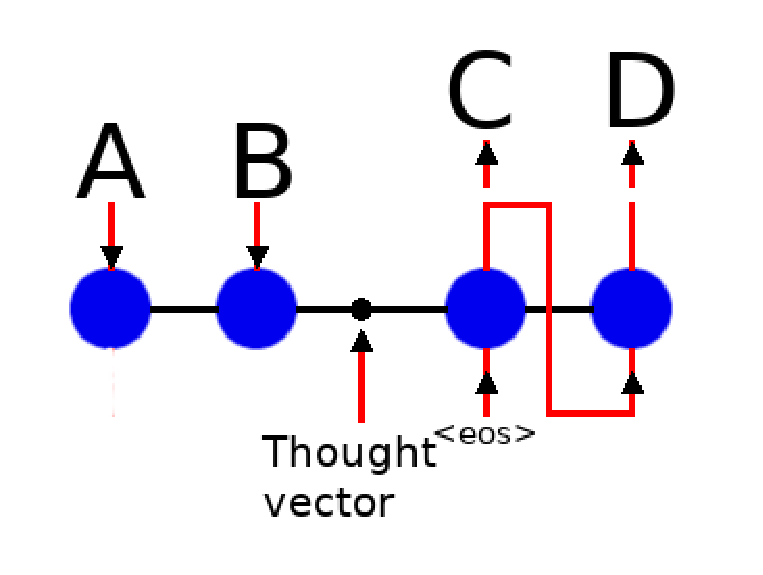
\includegraphics[scale=0.5]{diagram-nmt}

	
\end{center}

\caption[Sequnce to Sequence]{Seq2seq: A and B represent an input sequence and C and D represent the corresponding output.}

\end{figure}


\section{Sequence to Sequence Architecture}

In Fig. A.1 we generalize a sequence to sequence model. The idea is
that A and B, on the left side of the diagram, deal with the encoding
of sentences. A and B would be consecutive words in a sentence, and
the round blue nodes below A and B are RNN units. They are Recurrent
Neural Network elements. C and D are outputs and in the right side
of the diagram the blue nodes represent the output RNN units. Between
the input and the output there is a corridor of information exactly
the size of the RNN hidden vector. 

All of the information that the decoder uses for it\textquoteright s
output is present in this corridor and is passed along the corridor
from the encoder. For this reason we refer to it as the thought vector.

Making this vector larger by increasing the size of the hidden unit
size allows for more information in the thought vector. Size also
increases the time to train the network. The size must also match
the dimension of the vectors in the GloVe or Word2Vec download if
one of those is used. 

Ultimately exceedingly large hidden dimension does not improve the
sequence to sequence model. 



\section{Corpus Considerations}
We have collected several data sets for the training of a chatbot model. Firstly we have a corpus of movie subtitles.
Secondly we have the `JSON' dump from Reddit that is downloadable. Finally
we have the corpus described by Mazar{\'{e}} et al(2018)\cite{DBLP:journals/corr/abs-1809-01984}.
This final corpus is designed for training the chatbot task specifically. This is 
referred to as the Persona corpus.

The movie corpus is medium sized and the Reddit `JSON' download is large
and filled with hyperlinks and sentence fragments. 

At the time of
this writing we are using the movie subtitles corpus and the Persona corpus. We use the movie
corpus because it is smaller. Both the movie corpus and the Reddit
corpus are described as noise filled, so it is likely that neither
one is perfect for the training. The movie corpus is easier to deal
with if we are training on a single processor. In the future if we
can train in a faster environment the Reddit corpus might be superior.

For the Persona corpus the text is organized into `JSON' objects. There
are several different repeated labels. Some of the text is meant to be used in question and answer pairs. There is also some very specific information there that is not
organized in this kind of pattern. When we take apart the Persona corpus
we find that the sentences labeled with the `history' tag are most suited to our task.
We record these values only and discard other labels.



\section{Word Embeddings}

There are several basic building blocks of sequence to sequence models. 
They are regular neural network cells, recurrent
network components, and word embedding components.

Regular neural network cells, are arranged in layers and are pretty
straight forward in most programming environments. To use them you
define their dimensions in width and height. They have weights and
biases that must be initialized before use.

Recurrent networks have internal parts that are constructed of regular
network cells, so they have weights and biases too. They have several
internal dimensions that need to be set. One of these is the RNN hidden
unit. This hidden unit is a dimension.

Word embedding components are the third item we want to describe.
What happens is words are translated from strings to individual numbers
from a vocabulary dictionary. The dictionary only contains a single
unique number for every word. Then the number is passed through an
embedding structure. This turns the single number into a vector of
numbers that is the same size as the RNN hidden dimension. Then, from
that time on the model uses the vector instead of words.

The contents of the embedding unit is a table of numbers, all of the
size of the RNN hidden dimension. The vectors are usually, but don\textquoteright t
have to be, unique values. There is one complete hidden dimension
sized vector for each word in the vocabulary. 

\begin{figure}[H]
	\begin{center}
	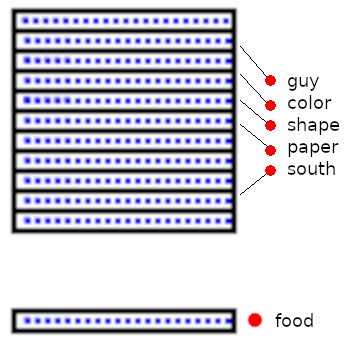
\includegraphics[scale=0.5]{diagram-embedding}
	
	
\end{center}
	\caption[Word Embeddings]{Embeddings: Each word from a dictionary is converted to a vector of numbers.}
	
	%\addcontentsline{lof}{section}{Word Embeddings}
\end{figure}

The vectors can be initialized randomly or they can be filled with
predetermined values. As the network trains the embedding values can
either be modified or frozen in place. Typically if the contents were
initialized randomly the values would be trained. If the contents
were filled with predetermined values you don\textquoteright t want
to train them or change them in any way. 

There are at this writing two main types of pretrained word embeddings.
One is called \textquoteleft Word2Vec\textquoteright{} and one is
called \textquoteleft GloVe\textquoteright . 

Word2Vec is short for \textquoteleft Word to Vector.\textquoteright{}
(Mikolov et al, 2013)\cite{mikolov2013efficient} GloVe is short for \textquoteleft Global
Vector.\textquoteright{} (Pennington et al, 2014)\cite{pennington-etal-2014-glove} .


\section{WordPiece - BPE}

\ac{BPE} stands for `Byte Pair Encoding.' WordPiece is a particular implementation of Byte Pair Encoding.

WordPiece is used by the BERT system to encode words much the way that Word2Vec does.
Like Word2Vec, WordPiece  has a vocabulary list and a table of embeddings that maps one
word or token to a vector of a given size.

WordPiece, though, handles Out Of Vocabulary (OOV) words gracefully. It breaks large words
into smaller pieces that are in the vocabulary, and has a special notation so that
these parts can easily be recombined in order to create the input word again.


\section{Transformer}

In this section we discuss the `Transformer' model. In their paper, Vaswani et al (2018)\cite{tensor2tensor} describe use of the python project Tensorflow and the Transformer model which is part of it.

The Transformer uses no recurrent elements. It is in a sense a group of attention mechanisms. The Transformer in this case is a single structure that can be used to solve many machine learning problems. It is used for Neural Machine Translation, Sentiment Analysis, and others. It is a single model capable of solving many machine learning questions.

We use the translation models for the chatbot problem by feeding the model the English language on both input and output. 

The Transformer itself can be configured for sentence long output but it is not a pre-trained model. There are pre-trained versions of the transformer, one of which is called BERT. BERT is described in Devlin et al (2018)\cite{DBLP:journals/corr/abs-1810-04805} and the acronym stands for Bidirectional Encoder Representations from Transformers. Unfortunately BERT output is as a 
classifier. Full sentence-length output is not supported.

\section{GPT2}

Another pre-trained model that uses the Transformer is GPT2. GPT2 stands for `Generative Pre-training Transformer 2.'

GPT2 is a model that takes as input a seed sentence or topic and returns as output text in the same language that is auto-generated. GPT2 also is very capable at summarizing the input or seed statement. We use both of these capabilities in our experiments.

There are two GPT2 models. One is larger than the other. The smaller model has been released and the larger model has not. 

GPT2 is discussed in Radford et al (2019)\cite{radford2019language} and on the blog associated with the parent company, OpenAI.com. (https://openai.com/blog/better-language-models/)

GPT2 comes with its own vocabulary encoding and decoding functionality. This system is closer to
WordPiece and BPE than it is to Glove or Word2Vec.

It is pre-trained on a corpus that is developed from Reddit posts called WebText. WebText is a
40 Gigabyte corpus that takes high powered computers to train.

The version of GPT2 which has been released is similar in size to the largest currently released 
BERT transformer model. GPT2 has been released in Tensorflow format, and more recently in a converted PyTorch format. It is possible to download the trained model and then fine-tune the model for your own task. This kind of fine-tuning is called `transfer learning'. 

GPT2 works so well in certain conditions that it is appropriate to use without fine tuning. This 
type of implementation is called `zero-shot' implementation. We use GPT2 in a zero-shot implementation with the chatbot problem.

\iffalse
\section{Question Answering -- GPT2}
To experiment with transfer learning on GPT2 we have completed a table of results for the babi
question answering problem. 

First we program our own version of the DMN project (Kumar et al, 2015)\cite{DBLP:journals/corr/KumarISBEPOGS15}. Then we try to
solve the same problem with GPT2. We achieve results for the 20 tests with accuracy in the mid to
high 90 percent. Our results are not higher than the hand coded version but they are respectable
and show the flexibility of the GPT2 model.
\fi

\section{Raspberry Pi}

A Raspberry Pi is a small single board computer with an `arm' processor. There are 
several versions on the market, the most recent of which sports built-in wifi and
on-board graphics and sound. The memory for a Raspberry Pi 3B computer is 1Gig of RAM. Recently
available, the Raspberry Pi 4B computer can sport 4Gig of RAM.

It has always been the intention that at some time some chatbot of
those examined will be seen as superior and will be installed and
operated on a Raspberry Pi computer. If more than one model is available
then possibly several models could be installed on Pi computers.

For this to work several resources need to be made available. Pytorch
needs to be compiled for the Pi. Speech Recognition (SR) and Text
To Speech (TTS) need to work on the Pi.

For the transformer model to work Tensorflow needs to work on the Pi.

All the files that are trained in the chosen model need to be small
enough in terms of their file size to fit on the Pi. Also it must
be determined that the memory footprint of the running model is small
enough to run on the Pi.

In the github repository files and scripts for the Raspberry Pi are
to be found in the \textquoteleft bot\textquoteright{} folder.

Early tests using Google\textquoteright s SR and TTS services show
that the Pi can support that type of functionality. 

Google's SR service costs money to operate. Details
for setting up Google's SR and TTS functions is beyond
the scope of this document. Some info about setting this up can be
found in the README file of this project\textquoteright s github
repository.

The pytorch model that is chosen as best will be trained on the
desktop computer and then the saved weights and biases will be transferred
to the Raspberry Pi platform. The Pi will not need to do any training,
only inference. 



\section{Speech}

Google has python packages that translate text to speech and speech to text. In the case of text
to speech the library is called `gTTS'. In the case of speech to text the library is called `google-cloud-speech'. 

The gTTS package is simple to use and can be run locally without connection to the internet. The google-cloud-speech package uses a google cloud server to take input from the microphone and 
return text. For this reason it requires an internet connection and an account with Google that
enables google cloud api use. Google charges the user a small amount for every word that they
translate into text. 

